\documentclass[letterpaper,11pt]{article}

\usepackage[margin=1.0in]{geometry}
\usepackage{amsmath}
\usepackage{amsthm}
\usepackage{amsfonts}
\usepackage{algorithm2e}
\usepackage{url}
\usepackage{fancyhdr}
\usepackage{blkarray}
\usepackage{graphicx}
\usepackage{csquotes}
\usepackage{cite}
\pagestyle{fancy}
\lhead{Algorithmic-Trading Summary --- Fall 2018}
\rhead{}


\begin{document}
\thispagestyle{plain}
\noindent{Algorithmic-Trading --- Fall 2018}

\noindent{Alex Thomas}

\noindent{Colgate University} \\

\noindent\textbf{Algorithmic-Trading - Bollinger Bands}

\section*{Introduction }

Bollinger Bands were introduced by John Bollinger in the 1980s. They provide a relative definition for high and low stock prices. This strategy uses 3 bands, with the 2 outer bands derived from a std deviation of the moving average. This is a momentum trading strategy, as the closing price moving between each band creates different buy or sell incentives. 

\section*{Motivations and Measures}

Bollinger bands are great measures of market conditions of a particular security. Just like the previously examined techniques, the method uses a simple moving average for its middle band. The upper and lower bands are separated by the a positive and negative difference in std deviations using the middle band as a base. Precisley, the upper band is calculated by adding $2 * $period standard deviation and the lower by subtracting this amount. Because of this use of standard deviation, which is determined by market volatility, Bollinger Bands adjust themselves to market conditions. When the market is more volatile the bands widen and when the market becomes less erratic, the bands move closer together \cite{Liu2006}. Unlike the previous techniques, this strategy uses market conditions to evaluate trading orders.

\section*{Key Techniques}

This strategy is implemented with these 3 bands as mentioned above. For our implementation, a 12 day window was chosen to test out the algorithm, as this has been proven to be the most effective \cite{Liu2006}. When the closing price drops below the lower band, this gives a buy signal, as once a lower band has been broken due to heavy selling, the stock price will revert back and head towards the middle band. The opposite is true for when the closing price breaks the upper band, as this is indicative of heavy buying. The closing price approaching the upper band gives a bearish signal while when it approaches the lower band this gives a bullish signal.

\begin{figure}[ht!]
\centering
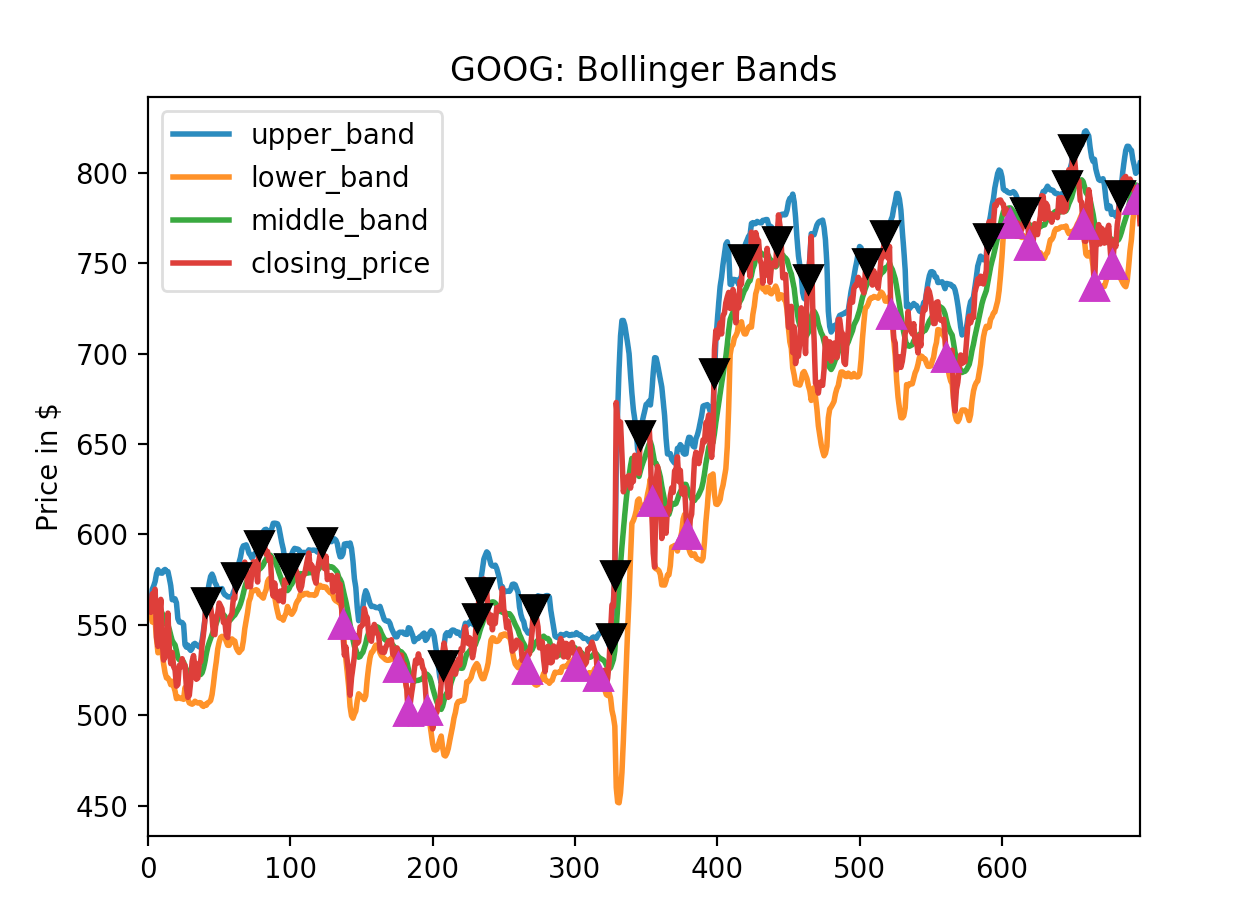
\includegraphics[width=90mm]{Goog_Bbands.png}
\caption{Bollinger Bands strategy applied to GOOG  \label{overflow}}
\end{figure}

\section*{Analysis}

\subsection*{Effectiveness}
Similar to our previous strategies, buy and sell signals are reliant on changes in rolling average prices. However, because of the incorporation of standard deviation, this strategy uses volatility in the market to further base buy and sell decisions. See Figure 1 to see how the strategy works.

\subsection*{Runtime}
The components to consider for this strategy include pulling stock data into a Pandas data frame and calculating rolling means from the data-frame and marking their differences. Pandas is a python data analysis package and is perhaps the most powerful open source data analysis or manipulation tool available. For each calculation, it has to scrape through the entire data-frame at a rolling window, giving a linear runtime.

\subsection*{Quality Metric}
The strategy is tested against a baseline long position of 100 shares of a given stock. Therefore, we compare the strategy against simply buying 100 shares of stock right at the opening date and then sell at the final date. For our implementation, over 15 different stocks were chosen and run against this baseline. TBD?

\subsection*{Space / Memory implications}
The only space for Bollinger Bands required is the data-frame, which is very reasonable.

\section*{Conclusion}
TBD once quality metric is implemented

\section*{Implementation}
\begin{verbatim}
def execute(stock, start_date, end_date):
    stock = stockDataRetriever(stock, start_date, end_date).getStock()

    # Initialize the short and long windows and buy sell in df
    window = 12

    # set Pandas df with stock data
    df = pd.DataFrame(index=stock.index)

    # Create short and long simple moving average
    df['middle_band] = df.sma(window)
    df['moving_deviation'] = df.std(window)
    df['upper_band'] = df['middle_band'] + df['moving_deviation'] * 2
    df['lower_band'] = df['middle_band'] - df['moving_deviation'] * 2

    # mark signal based on comparison of the two averages
    df[signal] = df.compare((df_closing_price, df_lower band), 
    		     (df_closing_price, df_upper_band),1,0)

    # when signal changes from 1 to 0 or 0 to 1 - is a buy or sell
    df[positions] = df[signal].diff()

\end{verbatim}

\bibliographystyle{plain}
\bibliography{References}

\end{document}